\documentclass[xelatex,aspectratio=169]{beamer}

\hfuzz=10pt
\vfuzz=10pt

% Theme
\usetheme{htw}
\setbeamertemplate{navigation symbols}{}
\setbeamertemplate{theorems}[numbered]
\setbeamercovered{transparent}

%\logo{
\includegraphics[height=0.5cm]{HTWD_color.png}}

% Packages
\usepackage{polyglossia}
\setmainlanguage{german}
\setotherlanguage{english}

\usepackage[bigfiles]{pdfbase}
\ExplSyntaxOn
\NewDocumentCommand\embedvideo{smm}{
\group_begin:
\leavevmode
\tl_if_exist:cTF{file_\file_mdfive_hash:n{#3}}{
  \tl_set_eq:Nc\video{file_\file_mdfive_hash:n{#3}}
}{
  \IfFileExists{#3}{}{\GenericError{}{File~`#3'~not~found}{}{}}
  \pbs_pdfobj:nnn{}{fstream}{{}{#3}}
  \pbs_pdfobj:nnn{}{dict}{
    /Type/Filespec/F~(#3)/UF~(#3)
    /EF~<</F~\pbs_pdflastobj:>>
  }
  \tl_set:Nx\video{\pbs_pdflastobj:}
  \tl_gset_eq:cN{file_\file_mdfive_hash:n{#3}}\video
}
%
\pbs_pdfobj:nnn{}{dict}{
  /Type/RichMediaInstance/Subtype/Video
  /Asset~\video
  /Params~<</FlashVars (
  source=#3&
  skin=SkinOverAllNoFullNoCaption.swf&
  skinAutoHide=true&
  skinBackgroundColor=0x5F5F5F&
  skinBackgroundAlpha=0.75
  )>>
}
%
\pbs_pdfobj:nnn{}{dict}{
/Type/RichMediaConfiguration/Subtype/Video
/Instances~[\pbs_pdflastobj:]
}
%
\pbs_pdfobj:nnn{}{dict}{
/Type/RichMediaContent
/Assets~<<
/Names~[(#3)~\video]
>>
/Configurations~[\pbs_pdflastobj:]
}
\tl_set:Nx\rmcontent{\pbs_pdflastobj:}
%
\pbs_pdfobj:nnn{}{dict}{
  /Activation~<<
  /Condition/\IfBooleanTF{#1}{PV}{XA}
  /Presentation~<</Style/Embedded>>
  >>
  /Deactivation~<</Condition/PI>>
}
%
\hbox_set:Nn\l_tmpa_box{#2}
\tl_set:Nx\l_box_wd_tl{\dim_use:N\box_wd:N\l_tmpa_box}
\tl_set:Nx\l_box_ht_tl{\dim_use:N\box_ht:N\l_tmpa_box}
\tl_set:Nx\l_box_dp_tl{\dim_use:N\box_dp:N\l_tmpa_box}
\pbs_pdfxform:nnnnn{1}{1}{}{}{\l_tmpa_box}
%
\pbs_pdfannot:nnnn{\l_box_wd_tl}{\l_box_ht_tl}{\l_box_dp_tl}{
  /Subtype/RichMedia
  /BS~<</W~0/S/S>>
  /Contents~(embedded~video~file:#3)
  /NM~(rma:#3)
  /AP~<</N~\pbs_pdflastxform:>>
  /RichMediaSettings~\pbs_pdflastobj:
  /RichMediaContent~\rmcontent
}
\phantom{#2}
\group_end:
}
\ExplSyntaxOff


\usepackage{graphicx}
\usepackage[export]{adjustbox}
\usepackage{animate}
%\usepackage[dvipdfmx]{movie15_dvipdfmx}
\usepackage{media9}
\usepackage{tabularx}
\usepackage{colortbl}
\usepackage{booktabs}
\usepackage{makecell}
\usepackage{ltablex}
\usepackage{array}
\usepackage{multirow}
\usepackage{amsmath}
\usepackage{amsthm}
%\renewcommand{\arraystretch}{1.5}
\newcolumntype{L}[1]{>{\raggedright\let\newline\\\arraybackslash\hspace{0pt}}p{#1}}
\newcolumntype{C}[1]{>{\centering\let\newline\\\arraybackslash\hspace{0pt}}p{#1}}
\newcolumntype{R}[1]{>{\raggedleft\let\newline\\\arraybackslash\hspace{0pt}}p{#1}}
%\renewcommand\thesatz{\arabic{section}.\arabic{theorem}}
\makeatletter
\@addtoreset{theorem}{lecture}
\makeatother

\newtheorem{satz}{Satz}[section]
\newtheorem{lem}{Lemma}[section]
\newtheorem{beh}{Behauptung}[section]
\newtheorem{define}{Definition}[section]
\numberwithin{equation}{section}
\usepackage{ragged2e}
\usepackage{etoolbox}

\usepackage{color}
\usepackage{colortbl}
\definecolor{hellgrau}{rgb}{0.85,0.85,0.85}
\definecolor{hellrot}{rgb}{1,0.7,0.7}

\usepackage{tikz}
\usetikzlibrary{shapes,arrows.meta,calc,arrows,positioning,patterns,tikzmark}
%\usepackage{tikz-uml}
\usepackage{pgfplots}  % for elliptic curves (part 8)
\pgfplotsset{compat=1.18}
\usepackage{pgffor}
\usepackage{pgfmath-xfp}
\tikzset{>=latex}
\tikzset{
  invisible/.style={opacity=0},
  visible on/.style={alt={#1{}{invisible}}},
  alt/.code args={<#1>#2#3}{%
      \alt<#1>{\pgfkeysalso{#2}}{\pgfkeysalso{#3}} % \pgfkeysalso doesn't change the path
    },
}

\usepackage{paralist}

\usepackage{url}
\def\UrlBreaks{\do\/\do-}
\PassOptionsToPackage{hyphens}{url}\usepackage{hyperref}

\usepackage[normalem]{ulem} % gestrichelte Unterstreichung (\dashuline{})
\usepackage{cancel}

\makeatletter
\renewcommand{\itemize}[1][]{%
  \beamer@ifempty{#1}{}{\def\beamer@defaultospec{#1}}%
  \ifnum \@itemdepth >2\relax\@toodeep\else
    \advance\@itemdepth\@ne
    \beamer@computepref\@itemdepth% sets \beameritemnestingprefix
    \usebeamerfont{itemize/enumerate \beameritemnestingprefix body}%
    \usebeamercolor[fg]{itemize/enumerate \beameritemnestingprefix body}%
    \usebeamertemplate{itemize/enumerate \beameritemnestingprefix body begin}%
    \list
    {\usebeamertemplate{itemize \beameritemnestingprefix item}}
    {\def\makelabel##1{%
        {%
            \hss\llap{{%
                  \usebeamerfont*{itemize \beameritemnestingprefix item}%
                  \usebeamercolor[fg]{itemize \beameritemnestingprefix item}##1}}%
          }%
      }%
    }
  \fi%
  \beamer@cramped%
  \justifying% NEW
  %\raggedright% ORIGINAL
  \beamer@firstlineitemizeunskip%
}
\makeatother

\apptocmd{\frame}{}{\justifying}{}

\renewcommand\theadfont{\bfseries\sffamily}
\usepackage{ragged2e}
\usepackage{newpxtext}

\setsansfont{texgyreheros}[
  Scale=MatchLowercase,
  UprightFont=*-regular,
  BoldFont=*-bold,
  ItalicFont=*-italic,
  BoldItalicFont=*-bolditalic,
]

% Title
\usepackage[usetransparent=false]{svg}
% Import references
\usepackage[backend=biber,style=numeric,sorting=none]{biblatex}
\addbibresource{references.bib}

%\AtBeginSection[]{
%  \begin{frame}
%    \vfill
%    \centering
%    \begin{beamercolorbox}[sep=8pt,center,shadow=true,rounded=true]{title}
%      \usebeamerfont{title}\thesection.~\secname\par%
%    \end{beamercolorbox}
%    \vfill
%  \end{frame}
%}

\makeatletter
\newenvironment{noheadline}{
  \setbeamertemplate{headline}{}
  \addtobeamertemplate{frametitle}{\vspace*{-0.9\baselineskip}}{}
}{}
\makeatother


\usepackage{xcolor}
\usepackage{algorithm}
\usepackage[linesnumbered,ruled,lined,commentsnumbered,algo2e,ngerman,ngermankw]{algorithm2e}
\usepackage{algorithmic}
\usepackage{caption}
\usepackage[newfloat]{minted}
\captionsetup[listing]{position=top}
\definecolor{mintedbg}{HTML}{282828}
\setminted{
  breaklines=true,
  bgcolor=mintedbg,
  style=monokai,
  formatcom=\color{white}
}
\usepackage{etoolbox}
\makeatletter
% replace \medskip before and after the box with nothing, i.e., remove it
\patchcmd{\minted@colorbg}{\medskip}{}{}{}
\patchcmd{\endminted@colorbg}{\medskip}{}{}{}
\makeatother

\renewcommand{\theFancyVerbLine}{\textcolor{black}{\arabic{FancyVerbLine}}}

\usepackage{pifont}
\newcommand{\cmark}{\ding{51}}%
\newcommand{\xmark}{\ding{55}}%

\newenvironment{changemargin}[2]{%
  \begin{list}{}{%
      \setlength{\topsep}{0pt}%
      \setlength{\leftmargin}{#1}%
      \setlength{\rightmargin}{#2}%
      \setlength{\listparindent}{\parindent}%
      \setlength{\itemindent}{\parindent}%
      \setlength{\parsep}{\parskip}%
    }%
    \item[]}{\end{list}}


\usepackage{csquotes}

% Title
\title{Einführung in Python}
\author{Prof. Dr. Lukas Iffländer}
\institute{HTW Dresden}
\date{}
\usepackage{svg}

% Begin document
\begin{document}

% Title slide
\begin{frame}
  \titlepage
\end{frame}


\begin{frame}{Warum Python?}
  
\includegraphics[width=.3\linewidth]{img/python_logo.png}
  \begin{itemize}
    \item Einfach zu lernen
    \item Vielseitig einsetzbar
    \item Große Community
    \item Viele Bibliotheken
    \item Open Source
    \item Hohe Nachfrage nach Python-Entwicklern
    \item Ideal für Datenanalyse und Machine Learning
  \end{itemize}
\end{frame}

\begin{frame}{Hello world in Python}
  Wir erstellen mit einem Texteditor (Notepad, Kate, Gedit) eine Pythondatei mit folgendem Inhalt:

  \begin{listing}
    \caption{hello\_world.py}
    \inputminted{python}{src/hello_world.py}
  \end{listing}

  Wir führen das Script aus, indem wir in der Konsole \texttt{python hello\_world.py} eingeben:

  \only<1>{\inputminted{console}{src/hello_world_pre}}

  \only<2->{\inputminted{console}{src/hello_world_post}}

  \only<3>{Auf diese Art und Weise können beliebige Python-Programme erstellt und ausgeführt werden.}

\end{frame}

\begin{frame}{Python-Programme werden interpretiert}
  \begin{block}{Unterschiede zu kompilierten Sprachen}
    \begin{itemize}
      \item Python-Programme werden nicht kompiliert, sondern interpretiert
      \item Der Python-Interpreter führt den Code Zeile für Zeile aus
      \item Fehler werden erst zur Laufzeit erkannt
      \item Python-Programme sind plattformunabhängig
    \end{itemize}
  \end{block}

  Python kann auch interaktiv genutzt werden. Dazu starten wir den Python-Interpreter mit dem Befehl \texttt{python}:

  \only<1>{\inputminted{console}{src/python_interactive0}}
  \only<2>{\inputminted{console}{src/python_interactive1}}
  \only<3>{\inputminted{console}{src/python_interactive2}}

\end{frame}

\begin{frame}{Gesprächiger: ipython}
  Zum Testen gibt es einen etwas gesprächigeren Interpreter namens \texttt{ipython}. Das \enquote{i} steht dabei für \enquote{interactive}.

  \only<1>{\inputminted{console}{src/ipython_interactive1}}
  \only<2>{\inputminted{console}{src/ipython_interactive2}}
  \only<3>{\inputminted{console}{src/ipython_interactive3}}
\end{frame}

\begin{frame}[plain,t]{Spyder Overview}
  \vspace{-.65cm}
  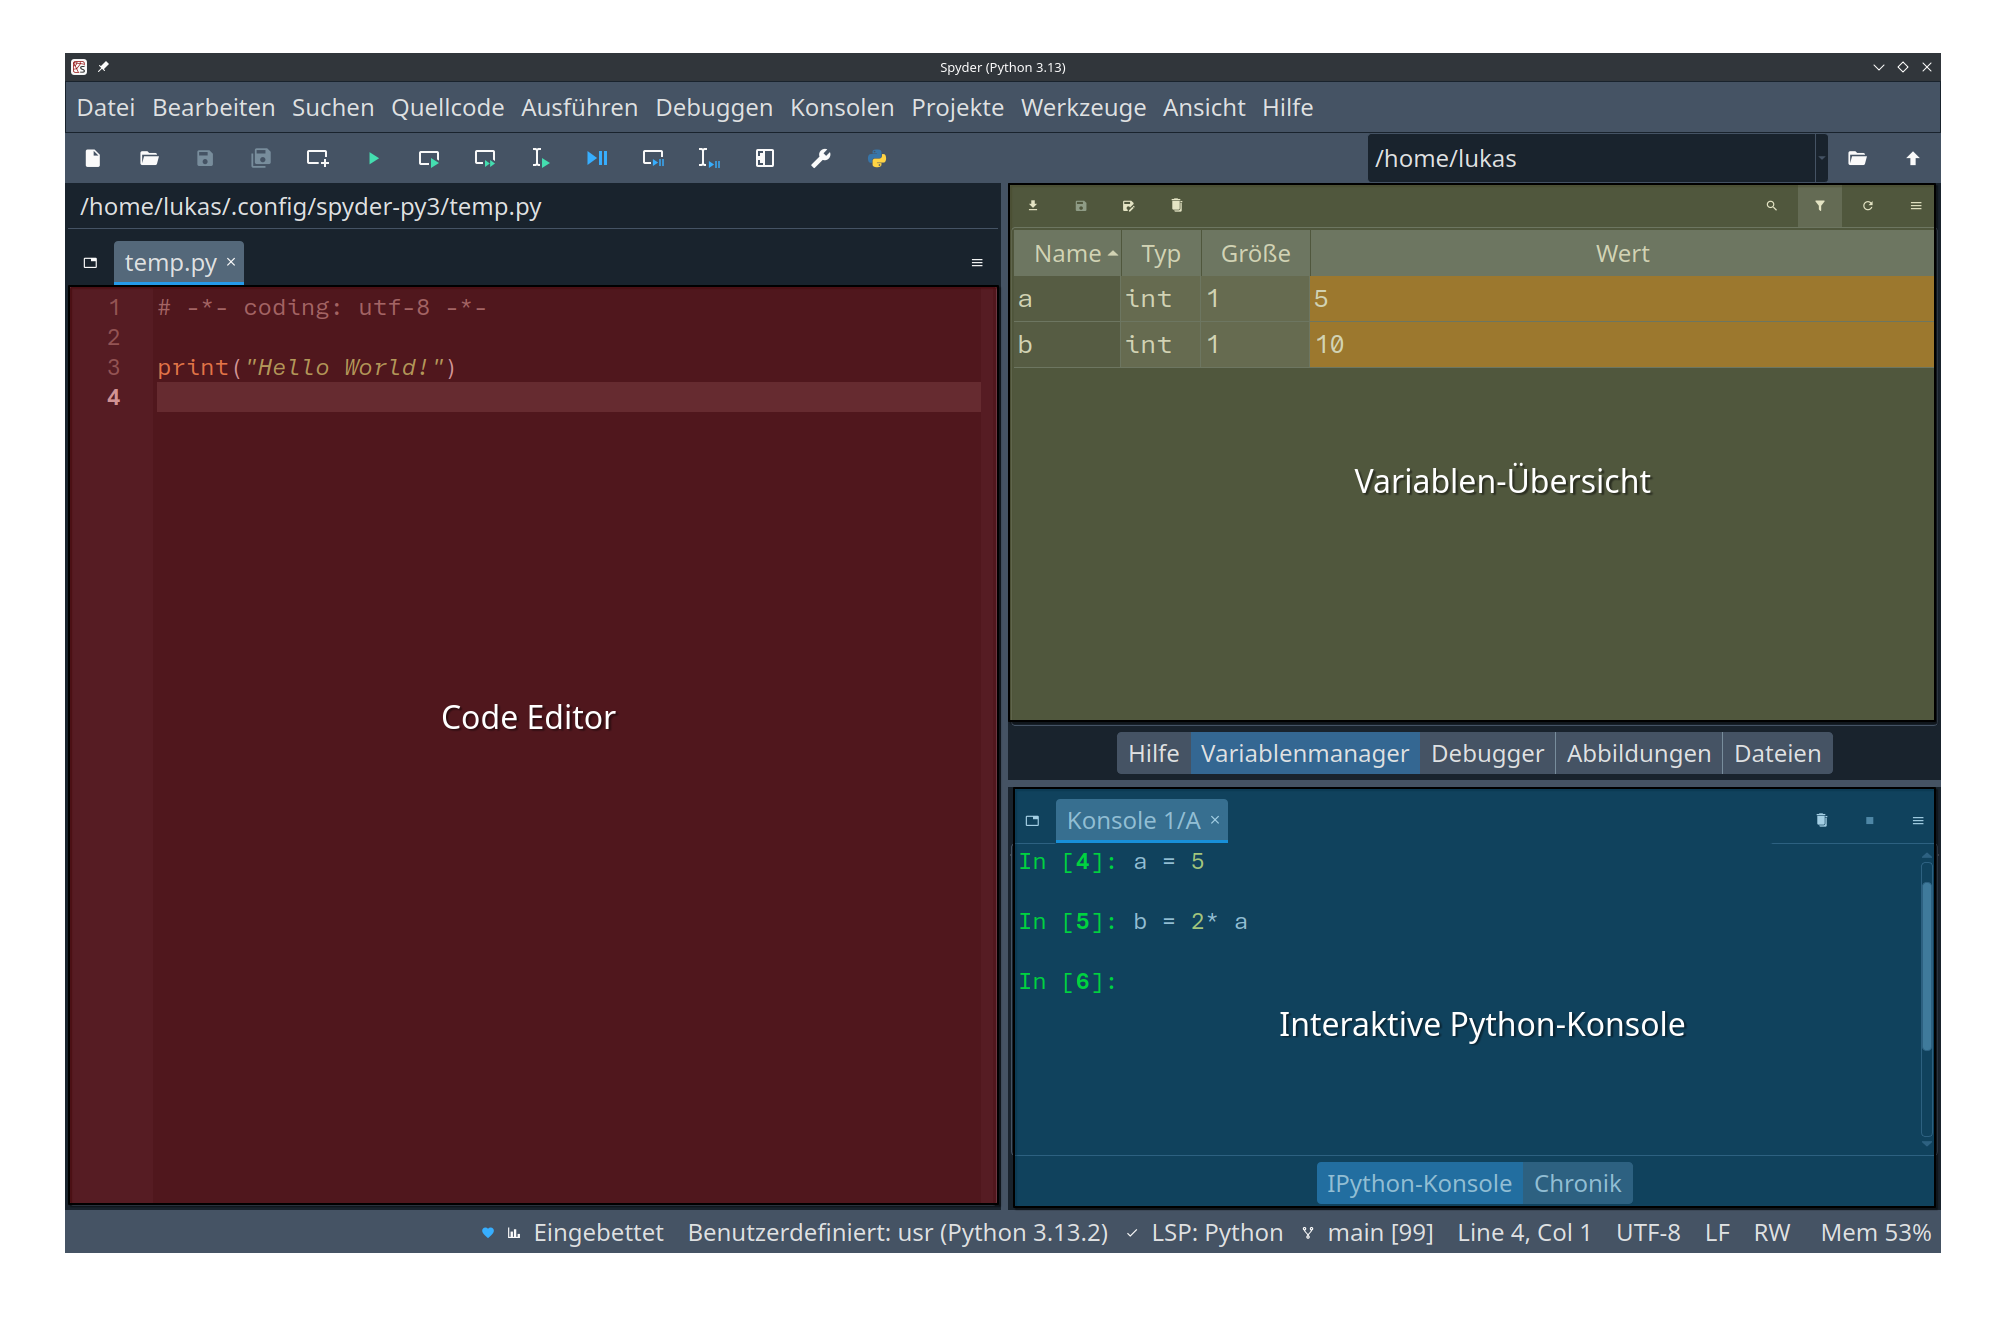
\includegraphics[height=\paperheight]{img/spyder_overview.png}
\end{frame}

\begin{frame}{Programme und Scripts}
  \begin{block}{Python-Scripts}
    Python-Skripts sind Textdateien, die Anweisungen enthalten,
    die schrittweise vom Python-Interpreter ausgeführt werden.
  \end{block}

  \begin{block}{Python-Programme}
    Python-Programme sind auch Skripte, sind aber komplexer,
    z.B. bestehen aus mehreren Python-Dateien (Module).
  \end{block}
\end{frame}

\begin{frame}{Wie programmiert man in Python}
  \begin{block}{Interaktive Programmierung}
    \begin{itemize}
      \item Umsetzen von Rechenoperationen und Ausdrücken in der Python-Shell.
      \item Ideal zum Ausprobieren und Testen von Code.
    \end{itemize}
  \end{block}
  \begin{block}{Skripte und Programme im Editor schreiben}
    \begin{itemize}
      \item Python-Code in einer Textdatei speichern.
      \item Für Programme, die öfter ausgeführt werden sollen.
    \end{itemize}
  \end{block}
\end{frame}

\begin{frame}{Einfaches Mathe}
  \begin{columns}
    \begin{column}{.25\linewidth}
      \inputminted{python}{src/math_example.py}
    \end{column}
    \begin{column}{.8\linewidth}
      \inputminted{console}{src/math_example_interactive}
    \end{column}
  \end{columns}
\end{frame}

\begin{frame}{Mehr Mathe ist schon fertig}
  \inputminted{python}{src/math_libraries.py}
\end{frame}

\begin{frame}{Arithmetische Operatoren}
  \begin{table}[]
    \begin{tabular}{cll}
      \toprule
      \textbf{Operator} & \textbf{Beschreibung} & \textbf{Beispiel}    \\ \midrule
      \texttt{+}        & Addition              & \texttt{2 + 3 = 5}   \\
      \texttt{-}        & Subtraktion           & \texttt{5 - 2 = 3}   \\
      \texttt{*}        & Multiplikation        & \texttt{2 * 3 = 6}   \\
      \texttt{/}        & Division              & \texttt{6 / 3 = 2.0} \\
      \texttt{//}       & Ganzzahldivision      & \texttt{7 // 3 = 2}  \\
      \texttt{\%}       & Modulo                & \texttt{7 \% 3 = 1}  \\
      \texttt{**}       & Potenz                & \texttt{2 ** 3 = 8}  \\ \bottomrule
    \end{tabular}
  \end{table}
\end{frame}

\begin{frame}{Zuweisungsoperatoren}
  \vspace{-12pt}
  \begin{table}[]
    \small
    \begin{tabular}{clll}
      \toprule
      \textbf{Operator} & \textbf{Beschreibung}            & \textbf{Beispiel}      & \textbf{Äquivalent}          \\
      \midrule
      \texttt{=}        & Zuweisung                        & \texttt{a = b}         & \texttt{-           }        \\
      \texttt{+=}       & Addition und Zuweisung           & \texttt{a += b}        & \texttt{a = a + b   }        \\
      \texttt{-=}       & Subtraktion und Zuweisung        & \texttt{a -= b}        & \texttt{a = a - b   }        \\
      \texttt{*=}       & Multiplikation und Zuweisung     & \texttt{a *= b}        & \texttt{a = a * b   }        \\
      \texttt{/=}       & Division und Zuweisung           & \texttt{a /= b}        & \texttt{a = a / b   }        \\
      \texttt{\%=}      & Modulo und Zuweisung             & \texttt{a \%= b}       & \texttt{a = a \% b  }        \\
      \texttt{//=}      & Ganzzahldivision und Zuweisung   & \texttt{a //= b}       & \texttt{a = a // b  }        \\
      \texttt{**=}      & Potenzierung und Zuweisung       & \texttt{a **= b}       & \texttt{a = a ** b  }        \\
      \texttt{\&=}      & Bitweises UND und Zuweisung      & \texttt{a \&= b}       & \texttt{a = a \& b  }        \\
      \texttt{$|$=}     & Bitweises ODER und Zuweisung     & \texttt{a $|$= b}      & \texttt{a = a $|$ b }        \\
      \texttt{\^{}=}    & Bitweises XOR und Zuweisung      & \texttt{a \^{}= b}     & \texttt{a = a \^{} b}        \\
      \texttt{>>=}      & Rechtsverschiebung und Zuweisung & \texttt{a >>= b}       & \texttt{a = a >> b  }        \\
      \texttt{<<=}      & Linke Verschiebung und Zuweisung & \texttt{a <<= b}       & \texttt{a = a << b  }        \\
      \texttt{:=}       & Zuweisung in Ausdrücken          & \texttt{print(a := b)} & \texttt{x = 3           }    \\
                        &                                  &                        & \texttt{print(x)           } \\
      \bottomrule
    \end{tabular}
  \end{table}
\end{frame}

\begin{frame}{Vergleichsoperatoren}
  \vspace{-12pt}
  \begin{table}[]
    \small
    \begin{tabular}{clll}
      \toprule
      \textbf{Operator} & \textbf{Beschreibung} & \textbf{True Beispiel} & \textbf{False Beispiel} \\
      \midrule
      \texttt{==}       & Gleichheit            & \texttt{2 == 2}        & \texttt{2 == 3}         \\
      \texttt{!=}       & Ungleichheit          & \texttt{2 != 3}        & \texttt{2 != 2}         \\
      \texttt{>}        & Größer als            & \texttt{3 > 2}         & \texttt{2 > 3}          \\
      \texttt{<}        & Kleiner als           & \texttt{2 < 3}         & \texttt{3 < 2}          \\
      \texttt{>=}       & Größer oder gleich    & \texttt{3 >= 3}        & \texttt{2 >= 3}         \\
      \texttt{<=}       & Kleiner oder gleich   & \texttt{2 <= 3}        & \texttt{3 <= 2}         \\
      \bottomrule
    \end{tabular}
  \end{table}
\end{frame}

\begin{frame}{Ausgabe}
  \begin{block}{\texttt{print()}-Funktion}
    \begin{itemize}
      \item Ausgabe der Werte aller Argumente in deren Reihenfolge
      \item Zwischen den Ausgaben werden Leerzeichen eingefügt
    \end{itemize}
  \end{block}
  \begin{exampleblock}{Beispiel}
    \inputminted{python}{src/print_komma_example.py}
    Output:
    \inputminted{console}{src/print_komma_example_output}
  \end{exampleblock}
\end{frame}

\begin{frame}{Eingabe}
  \vspace{-7pt}
  \begin{block}{\texttt{input()-Funktion}}
    \begin{itemize}
      \item Die input() Funktion liest eine Texteingabe bis zum Abschluss mit Enter und gibt den Text als Zeichenkette zurück.
      \item Bei Eingabe von Zahlenwerten ist der Text in den gewünschten numerischen Typ umzuwandeln, hier \texttt{int(...)} oder \texttt{float(...)}
    \end{itemize}
  \end{block}

  \begin{exampleblock}{Beispiel}
    \inputminted{python}{src/input_example.py}
  \end{exampleblock}
\end{frame}

\begin{frame}{Zeichenketten aka Strings}
  \begin{block}{Zeichenketten}
    Zeichenkettenkonstante zur Initialisierung werden in einfache oder doppelte Hochkomma-Zeichen eingefasst, bspw. \texttt{'Hund'} oder \texttt{''Katze''}
  \end{block}
  \begin{exampleblock}{Beispiel}
    \inputminted{python}{src/string_example.py}
  \end{exampleblock}
\end{frame}

\begin{frame}[allowframebreaks]{Datentypen}
  Anders als in vielen Sprachen legt man den Datentyp in Python nicht explizit fest.

  Der Interpreter wählt den Datentyp:
  \begin{itemize}
    \item anhand von Konstanten und dem Typ der benutzten Variablen
    \item durch verwendete Operatoren
  \end{itemize}

  \begin{alertblock}{Vorsicht}
    Der Typ ergibt sich möglicherweise erst zur Laufzeit des Programms, d.h. kann nicht ohne weiteres vorhergesagt werden (Schwierigkeit bei der Fehlersuche, Programmverifikation)
  \end{alertblock}

  \begin{exampleblock}{Wichtige Datentypen}
    \begin{table}
      \begin{tabular}{ll}
        \toprule
        \textbf{Datentypkürzel} & \textbf{Beschreibung} \\
        \midrule
        int                     & Ganzzahl              \\
        float                   & Gleitkommazahl        \\
        str                     & Zeichenkette          \\
        bool                    & Boolescher Wert       \\
        \bottomrule
      \end{tabular}
    \end{table}
  \end{exampleblock}
\end{frame}

\begin{frame}[allowframebreaks]{Funktionen}
  Vergleichbar mit mathematischen Funktionen, die aus Argumenten Ergebniswerte berechnen, können in Python Funktionen definiert werden.

  \begin{block}{Funktionsformat}
    \inputminted{python}{src/funktion_definition.py}
  \end{block}

  Mit \texttt{return} wird die Funktion verlassen und optional ein Rückgabewert zurückgegeben.

  \small
  \begin{exampleblock}{Beispiel}
    \inputminted{python}{src/function_example.py}
  \end{exampleblock}

\end{frame}

% End document
\end{document}
